% 2021 全国乙卷理科第 23 题的作图网格（补充解题辅助图）。
% 原卷 PDF 第 2 页未附坐标网格；本图按 a=1 绘出 f(x)=|x-1|+|x+3| 与 y=6。
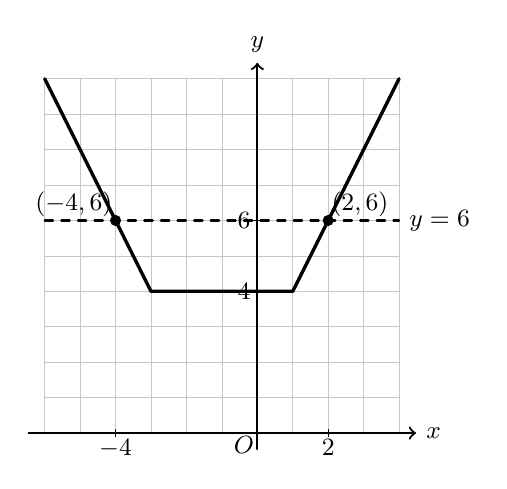
\begin{tikzpicture}[x=0.45cm,y=0.45cm,line cap=round,line join=round,font=\small]
  % Unit grid
  \draw[gray!45,line width=0.25pt] (-6,0) grid[step=1] (4,10);

  % Axes
  \draw[->,thick] (-6.45,0) -- (4.48,0) node[right] {$x$};
  \draw[->,thick] (0,-0.45) -- (0,10.45) node[above] {$y$};
  \node[below left,inner sep=1pt] at (0,0) {$O$};

  % Unit marks and the two boundary abscissas
  \foreach \x in {-4,2} {
    \draw (\x,0.10) -- (\x,-0.10);
    \node[below,inner sep=1pt] at (\x,-0.10) {$\x$};
  }
  \foreach \y in {4,6} {
    \draw (0.10,\y) -- (-0.10,\y);
    \node[left,inner sep=1pt] at (-0.10,\y) {$\y$};
  }

  % f(x)=|x-1|+|x+3| and the comparison level y=6
  \draw[dashed,thick] (-6,6) -- (4,6) node[right] {$y=6$};
  \draw[very thick] (-6,10) -- (-3,4) -- (1,4) -- (4,10);
  \fill (-4,6) circle (2pt);
  \fill (2,6) circle (2pt);
  \node[above right,inner sep=1pt] at (2,6) {$(2,6)$};
  \node[above left,inner sep=1pt] at (-4,6) {$(-4,6)$};
\end{tikzpicture}
